% !TEX root = ./memoire/main.tex
\chapter{Méthodes particulaires et assimilation de données}~\label{sec:prob_contribution}

\textcolor{red}{à compléter}
L'assimilation de données, lorsqu'elle est appliquée à des systèmes simulés par des méthodes lagrangiennes, se heurte à plusieurs limites importantes. A la fois pour les méthodes variationnelles (ex : 3DVar) ou stochastique (ex : EnKF) il faut considérer deux problématiques majeurs : la définition de l'état et la manière de le mettre à jour.
Nous évoquerons les singularités et limites à l'adaptation des méthodes d'assimilation de données. Cependant, ces problématiques trouvent un echo dans le reste de la littérature en particulier pour des problèmes à maillage adaptatif, lorsque les observations sont des données lagrangiennes ou lorsqu'une erreur de position doit être prise en compte. Finalement, nous présenterons la démarche de notre contribution.

\section{Problématique et revue bibliographique}

\subsection{Définition de l'état d'une méthode particulaire}~\label{sec:etat_meshless}

L'état est une représentation de toutes les variables pertinentes du système à un instant donné. Il est souvent représenté par un vecteur d'état $\bm z$ comme dans la Section~\ref{sec:da}. Pour les états continues, comme des champs de densité ou de vitesse dans notre cas, des méthodes de discrétisation sont utilisées. Elles sont essentielles pour la résolution numérique et permettent habituellement d'exprimer le vecteur d'état $\bm z$. Les méthodes classiques de simulation en mécanique vont utiliser un représentation fixe pour définir un espace de représentation fonctionnel.


On considère un domaine $\Omega \subset \mathbb R^d$, soit $\mathcal{T} = (\mathcal N, \mathcal E)$ un maillage, où $\mathcal N = \left\{\bm x_i \right\}^n_{i=1}$ est l'ensemble des nœuds, et $\mathcal{E} = \{ K_i \}_{i=1}^{m}$ l'ensemble des éléments.

\begin{itemize}

    \item \textbf{La méthode des éléments finis(FEM)}~\cite{fem} associe à chaque nœuds $i$ des fonctions de forme $\phi_i$.
          L'état de la solution \(u_h\) discrétisé peut alors être définie comme

          \begin{equation*}
              u_h(\bm x) = \sum_{i=1}^{N} u_i \phi_i(\bm x),
          \end{equation*}où $u_i$ les valeurs nodales à déterminer. Le vecteur d'état est défini sur les nœuds du maillage $\bz = \{ u(\mathbf{x}_1), \dots, u(\mathbf{x}_n)\}$

    \item \textbf{Méthode des volumes finis (FVM)}~\cite{fvm}, la solution est approximée par une valeur moyenne sur chaque élément $K_i$ comme

          \begin{equation*}
              u_i = \frac{1}{\lvert K_i \rvert}\sum_{i=1}^{m} \int_{K_i} u~\text{d}K
          \end{equation*}

          de telle sorte que la solution approchée est une solution constante par éléments

          \begin{equation*}
              u_h(\bm x) = \sum_i^m u_i \mathbb{1}_{K_i}(\bm x).
          \end{equation*}

          Il est alors possible de définir l'état comme une variable aléatoire  $\bz = \{ u(K_1), \dots, u(K_m)\}$.

    \item \textbf{méthode d'interpolation à fonctions de base radiale(RBF)} Tout comme les méthodes particulaire, la méthode d'interpolation RBF paramétrise les fonctions de base radiale $\phi$ par une position $\bm x_i$ et des paramètres de forme $\theta$ tel que

          \begin{equation*}
              u_h(\bm x) = \sum_{i}^n u_i \phi_i(\bm x; \bm x_i, \theta),
          \end{equation*}où $u_i = u(\bm x_i)$. Si $\phi$ est une fonction définie strictement positive, et $\bm x_i$ distinct, alors $u_h$ est bien défini de manière unique par les valeurs nodales. Ainsi l'état peut être défini comme $\bz = \{ u(\bm{x}_i) \}_{i=1}^{n}$
\end{itemize}

Les discrétisations étant fixes, il n'est pas nécessaire d'inclure la position des nœuds ou des éléments pour représenter l'état. Finalement, le modèle est résolu au cours du temps grâce à des équations différentielles tel qu'il est possible d'écrire $\frac{d \bm z}{dt}(t) = \mathcal M (\bm z(t); \mathcal D) $où $\mathcal D$ la discrétisation utilisée.

Dans le cas des méthodes lagrangiennes particulaires, la situation est différentes. En effet, Le support de discrétisation, porté par les particules, évolue également au cours du temps. L'état ne peut donc pas être défini uniquement par les valeurs d'intensité, mais doit considérer également les positions des particules.

Une première solution consiste à considérer chaque particules indépendamment dans la définition de l'état en associant position et intensité.

\begin{itemize}
    \item Pour la DEM, l'état à l’instant $t$, pourrait alors être défini comme
          \begin{equation*}
              \bz(t) = {(\bx_p(t), \bm v_p(t), \bm \theta_p(t), \bm \omega_p(t), A_p)}_{p=1}^N
          \end{equation*}où $N$ le nombre de grains, et présente à la fois les variables cinématiques ainsi que $A_i$ les propriétés intrinsèques de la particules comme sa masse ou sa géométrie.

    \item De même pour les méthodes particulaires continues, par exemple la méthode vortex, l'état peut être défini comme

          \begin{equation*}
              \bz = {(\bx_p(t),\bm \Gamma_p(t), A_p)}_{p=1}^{N_p}
          \end{equation*}où cette fois $A_i$ défini en particulier les propriétés de la fonction de lissage.
\end{itemize}

Dans ces cas, on peut en effet définir la fonction approchée $u_h$, et définir un modèle d'évolution pour l'état $\bm z$ comme décrit en Section~\ref{sec:simu_part}. Cette définition de l'état a en particulier été utilisé~\cite{chen_superfloe_2022} pour une méthode DEM appliquée au mouvement de la banquise ou bien avec la méthode vortex~\cite{darakananda_data-assimilated_2018,le_provost_ensemble_2021}. Ce sont des filtres EnKF qui ont été développés dans ces deux cas.

Toutefois, cette définition peut être assez contestable dans le cas général. Premièrement, il est alors nécessaire de faire l'hypothèse que tous les membres possèdent le même nombre de particules dans un ordre défini. Dans le cas contraire il n'est pas possible de réaliser le calcul des statistiques sur l'ensemble. Il est néanmoins possible d'ajouter des particules supplémentaires à la suite des précédentes dans le vecteur d'état en remplissant de valeurs nulles le cas échéant. Cependant, le risque est de voir le nombre de particules augmenter considérablement après mise à jour, ou de ne pas pouvoir représenter convenablement les statistiques de l'état discrétisé. Cette remarque est d'autant plus sensible en considérant le caractère chaotique d'un problème à N-corps~\cite{poincare1890}. En effet, dans ce cas, deux particules proches à une perturbation près peuvent, en un temps fini, voir leur trajectoires totalement décorrélée. Le système peut conserver une régularité dans sa globalité, mais il devient tout à fait incongru de continuer à comparer ces deux particules entre elles. Ainsi, il n'est plus possible de définir l'état comme selon une collection de particules individuelles ou bien de définir des statistiques qui est un sens pour une particule données.
%Finalement, pour les méthodes continues, on a une relation entre statistique du champ $u_h$ et état discret $\bm z$ qui est non linéaire. Par exemple, pour la moyenne
Dans les articles~\cite{chen_superfloe_2022} ou~\cite{darakananda_data-assimilated_2018} cette première limitation a été traité en regroupant les particules pour en obtenir des systèmes de plus faible dimension. Dans le premier cas, il s'agit de créer des superstructures de glace, dans le second cas, il s'agit d'utiliser des méthodes d'agglomération de vortex. L'assimilation de données est donc appliquée au détriment du niveau de détail des solutions.

En particulier, on obtient différent estimateurs Monte-Carlo avec les méthodes d'ensemble. En supposant un ensemble de champs $\{u_i\}_{i=1}^N$, de vecteur d'état associé $\left\{z_i = \left\{\bx_{ip},\bm \Gamma_{ip}\right\}_ {p \in \mathcal P}\right\}_{i=1}^N$, on obtient deux estimateurs Monte-Carlo pour la moyenne

\begin{eqnarray*}
    \mathbb{E}(u(\bm x)) \simeq e_1(\bm x) =\frac{1}{N} \sum_{i=1}^N u_i(\bm x) = \frac{1}{N} \sum_{i=1}^N \sum_{p \in \mathcal P}\bm \Gamma_{ip} \phi_\varepsilon(\bm x - \bx_{ip}), \\
    e_2(\bm x) = \sum_{p \in \mathcal P} \mathbb{E}(\bm \Gamma_{p}) \phi_\varepsilon\left(\bm x - \mathbb{E}(\bx_{p})\right) =\frac{1}{N} \sum_{i=1}^N \sum_{p \in \mathcal P} \bm \Gamma_{ip} \phi_\varepsilon(\bm x - \bar{\bx}_{p}),
\end{eqnarray*} où $ \bar{\bx}_{p} = \frac1N \sum_{i=1}^{N} \bx_{ip}$. Du fait de la non-linéarité du noyau, on obtient deux estimateurs différents.
\subsection{Mise à jour de l'état d'une simulation particulaire}

% \subsubsection{Pour les méthodes variationnelles}
Une autre problématique majeur est celle de la mise à jour de l'état lors de l'analyse. Une première limitation concerne les méthodes variationnelle comme la méthodes 3DVar présentée en~\ref{subsec:3dvar}. D'une part, l'opérateur d'observation $\mathcal H(z)$, est non-linéaire par rapport aux variables particulaires tel que la position $\bx_i$. Pour un système avec des milliers voire des millions de particules, on se retrouve à traiter un problème d'optimisation fortement non-linéaire dans un espace de très grande dimension. De nouveau, on pourrait procéder à une réduction du nombre de particules. Toutefois, dans le cas des méthodes discrètes, il est nécessaire de prendre en considération un nombre élevé de contraintes. Notamment, le déplacement des particules doit respecter l'interdiction d'interpénétration des particules. Cette conditions doit être vérifié sur l'ensemble du système pour assurer que la solution d'optimisation soit admissible. Dans le cas des méthodes continues, les particules sont des entités ponctuelles et ne représentent qu'une discrétisation d'un milieu continu. Ainsi cette dernière contrainte ne s'applique pas. Finalement, utiliser une méthode d'assimilation de données variationnelles dans le cas d'une discrétisation particulaire nécessite de traiter une problème d'optimisation non-linéaire de grande dimension avec contraintes pour la méthode DEM et sans contrainte dans le cas continu.

% \subsubsection{Pour la méthode EnKF}
Dans le cas de la méthode EnKF, la mise à jour est définie de manière statistique. De ce fait, elle ne tient pas compte de contraintes physiques. L'équation~\ref{eq:corr} montre en effet, que l'état estimé lors de l'analyse est une combinaison linéaire des états prédits par les différents membres de l'ensemble, en particulier sur les positions des particules $\bx_i$.
En DEM, bien que chaque membre vérifie les conditions de non interpénétration, ces conditions n'étant pas linéaire, il n'y a aucune garantie pour que la combinaison le soi. En d'autres terme, la mise à jour ne peut être réalisé que via le solveur lui-même capable de vérifier des contraintes de non interpénétration mais ne peut être réalisé directement. Dans le cas de l'article~\cite{chen_superfloe_2022}, si le filtre EnKF a pu être utilisé, c'est en parti car le critère non interpénétration est relaxé.

Si cette problématique ne concerne pas les méthodes particulaires continues, il reste toutefois questionnable de réaliser une combinaison linéaire des positions des particules. Cette question est en fait en lien avec la définition de l'état. En effet, chaque particule n'est que le support de la discrétisation d'un champ continu. Mesurer une erreur quadratique sur la position des particules n'aura pas de lien linéaire avec l'erreur quadratique sur le champ.

\textcolor{red}{Ceci est relativement vrai pour un champs d'un problème tournant. La rajouter une exemple, présente un cas où chaque membre discrétise un même champ de tourbillon mais où le support de discrétisation a plus ou moins de retard.}.
Encore une fois, une solution consiste à réaliser des agrégations pour regrouper les particules comme en~\cite{chen_superfloe_2022,darakananda_data-assimilated_2018} mais au détriment du détail de discrétisation.

% Finalement, la mise à jour en considérant des discrétisations particulaires est complexe. En DEM elle doit prendre en considération les positions relatives des particules entre elles. De manière générale, nous avons vu que considérer les statistiques sur les positions de particules ne permettait pas d'avoir une bonne idée de l'incertitude sur le champ discrétisé. Ainsi, il nous semble nécessaire de formuler différemment le problème d'assimilation dans le cadre d'un discrétisation particulaire pour tenir compte

Finalement, l'assimilation de données pour les méthodes particulaires souffre d'un certain nombre de limitations lié à la discrétisation lagrangienne de la solution. Pour les méthodes discrètes comme la DEM, la principale difficulté consiste à devoir prendre en compte les contraintes de distance entre particulaire, ce qui complique à la fois la mise à jour avec les méthodes stochastiques et variationnelles. De manière générale, il faut tenir compte de la variabilité dans les positions de la distribution particulaire. La non-linéarité de la solution par rapport aux positions limite l'applicabilité des méthodes classiques pour l'assimilation de données. Ainsi, il devient nécessaire de proposer des méthodes d'assimilation de données, qui soient adaptées au problème de discrétisation particulaire. D'une part, en considérant pour les méthodes ensemblistes, que chaque membre dispose d'une distribution de particule qui lui est propre. D'autre part, que le traitement de la mise à jour des positions et des intensités doit être différentiés.

\section{Revue bibliographique}

Ces limitations ne sont pas toute propre uniques à ce domaine, mais se retrouvent également dans d'autres disciplines. Le fait d'avoir un ensemble de membre ne partageant pas les mêmes discrétisations est aussi une problématique pour l'application du filtre EnKF avec des méthodes de maillages adaptatifs. De même, la même problématique de passé d'une représentation eulériennes, c'est à dire sur une grille fixe vers une représentation lagrangienne a également dû être considéré pour des observables. Finalement,

\subsection{Assimilation de données sur maillages adaptatifs}

Les méthodes particulaires continues peuvent être considérées comme le choix d'une discrétisation mobile d'un problème continu. Ainsi, en utilisant un ensemble de simulations basées sur ces méthodes, on se heurte aux mêmes problématiques que celles rencontrées avec des simulations utilisant des maillages adaptatifs.
Dans ce cas le principal défi réside dans le fait que les dimensions de l'espace d'état changent au cours du temps et diffèrent d'un membre de l'ensemble à l'autre. Cette variabilité complique les opérations ensemblistes habituelles, telles que les calculs matriciels, lors de la mise à jour de l'analyse.

Une solution courante consiste à adopter une discrétisation de référence commune à tous les membres. Dans les méthodologies à grille fixe avec l'analyse multi-résolution (MRA) et dans les scénarios de maillage mobile, les états définis sur des grilles variées sont harmonisés à travers des techniques de projection et d'interpolation pour établir une grille de référence destinée aux mises à jour des états \cite{siripatana_combining_2019, bonan_data_2017}. Cette démarche offre une grande flexibilité, permettant diverses combinaisons de grilles de référence et de mise à jour adaptées aux spécificités des données et des objectifs de l'étude. Par ailleurs, Siripatana et al. \cite{siripatana_combining_2019} soulignent que la correction par le Filtre de Kalman d’Ensemble (EnKF) repose uniquement sur les prédictions et les observations, indépendamment de la définition de l'état. En réalité, cela simplifie l'application de l'EnKF dans des contextes où les maillages varient entre les membres de l'ensemble en proposant une correction qui est indépendante de la discrétisation

\subsection{Méthodes d'assimilation pour des données lagrangiennes}
\textcolor{red}{présenter des méthodes dans des cas où les variables sont des quantités lagrangiennes}

D'autre part
- Méthodes particulaires sont des méthodes lagrangiennes
- Avoir données variable problématique déjà traité par des données océanographiques issu de flotteurs par exemple
- Pour traiter ce type de problème, une première approche initialement développé dans~\cite{ide_2002}, est d'augmenter le vecteur d'état ici noté $\bm x$ avec les données d'observation de position de traceur. Cependant, cette variable étant fortement non-linéaire, l'application d'un filtre de Kalman étendu (linéarisation du filtre de Kalman) ne converge pas si les observations ne sont pas suffisamment fréquente. Finalement, cela revient à définir l'état comme dans la Section~\ref{sec:etat_meshless} précédente, ce qui n'est pas adéquat.

L'utilisation d'une méthode de type état augmenté trouve plus de sens pour l'application de méthode variationnel.
C'est en particulier ce qui est proposé dans les travaux de Apte~\cite{apte_2008} pour le filtre 3DVar et le ceux de Nodet~\cite{nodet_2006} pour le filtre 4DVar incrémental.

Cependant, ici les quantités lagrangiennes sont des quantités passives, c'est à dire qu'elles n'interviennent pas dans la résolution du champ de vitesse à intégrer. Dans notre cas les traceurs sont des supports de discrétisation de la solution. De ce fait, le modèle adjoint du modèle n'est pas aussi simple à construire car la position des particules impactent le champ de vitesse à intégrer.


\subsection{Méthodes d'assimilation de données par déplacement ou alignement}~\label{sec:biblio_align}

Dans le Chapitre~\ref{sec:da}, nous avons présenté l'assimilation de données comme la combinaison les simulations issues d'un modèle avec les données bruités issues de l'observation. Cette combinaison nécessite de pouvoir mettre à jour de manière optimale l'état de la simulation en tenant compte à la fois de l'erreur \textit{a priori} du modèle ainsi que l'erreur d'observation. Plus précisément, ces méthodes cherchent à déterminer la distribution ou l'estimateur du maximum a posteriori (MAP) de l'état par correction de l'intensité.

Cependant, on trouve de nombreuses limitations à ces schémas classiques, en particulier lorsqu'il existe une erreur de position. En effet, les méthodes d'assimilation de données classiques sont construites en mesurant l'erreur à l'aide d'une norme quadratique qui tend à sur pénaliser des erreurs issues d'alignement. Pour s'en rendre compte, on peut constater en Figure~\ref{fig:double_penalization_error} qu'une erreur sur l'alignement sera sur-pénaliser en comparaison de l'erreur avec une solution nulle. On parle d'effet de \textit{double pénalisation} car cette effet intervient à la fois pour l'évaluation de l'erreur sur le modèle mais également sur les observations~\cite{amodei2009}. C'est d’ailleurs une des contribution majeur à l'erreur de représentativité~\cite{janjic2018}.

\begin{figure}[h]
    \centering
    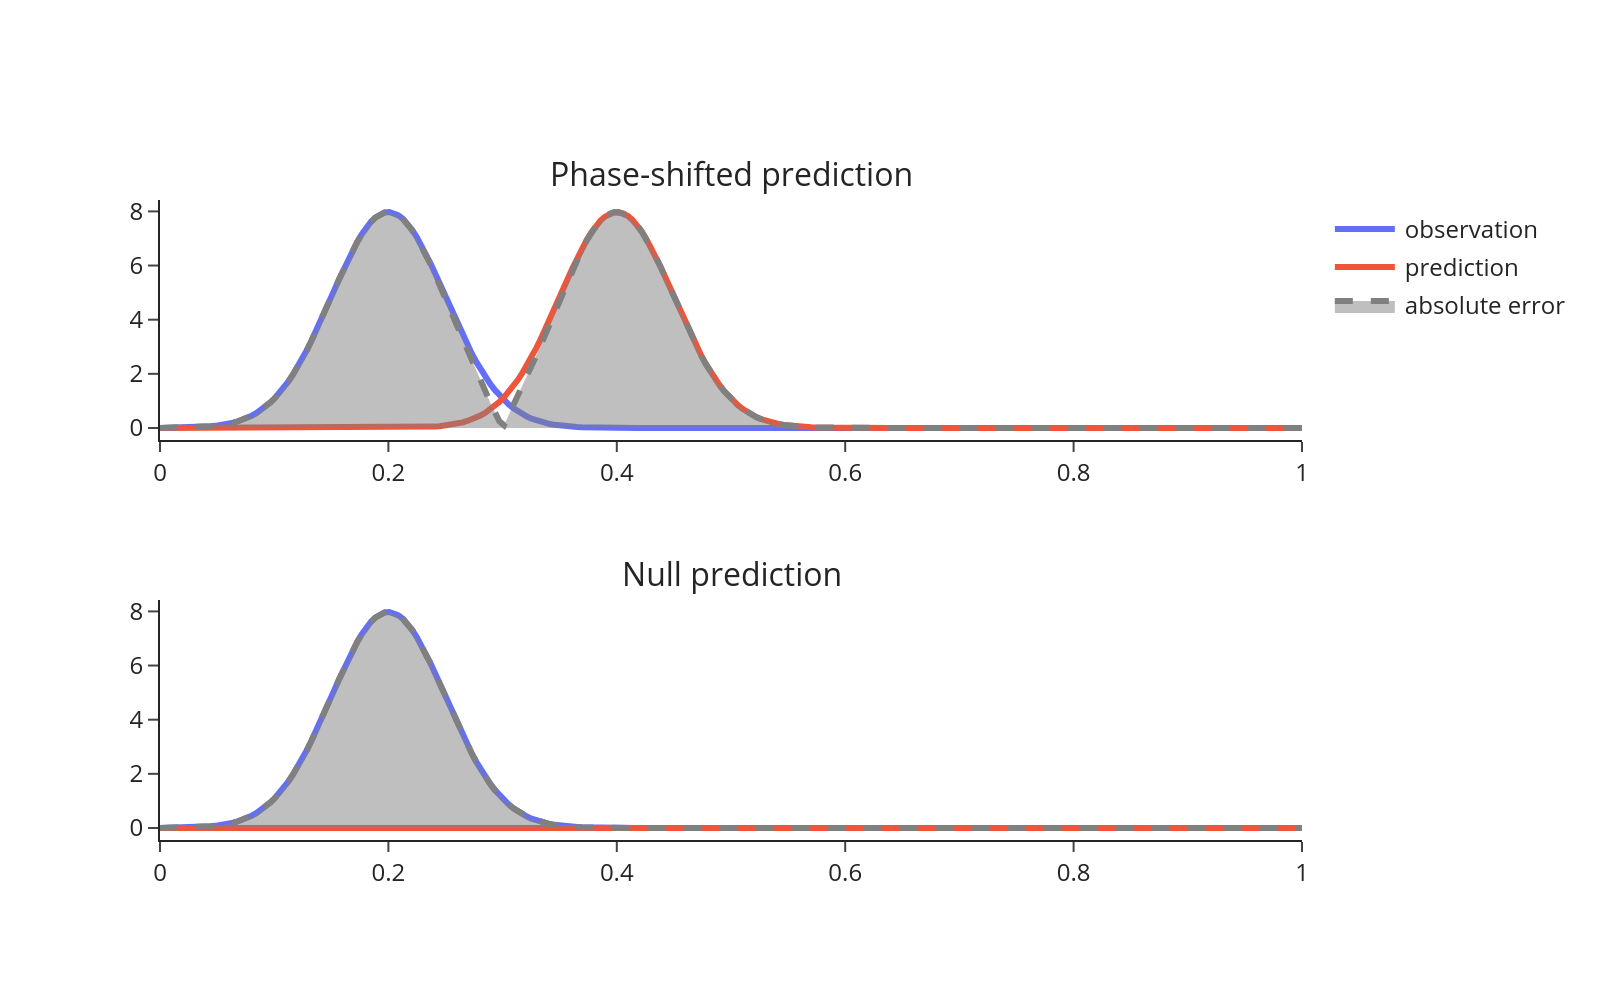
\includegraphics[width=\linewidth]{double_penalisation.png}
    \caption{Visualisation de l'effet de double pénalisation.}~\label{fig:double_penalization_error}
\end{figure}

Un seconde limitation, concerne la nécessité pour les champs d'état et d'observation \textit{a priori} de recouvrir la solution à analyser. En effet, la mise à jour des méthodes d'assimilation de données classique consiste essentiellement à un interpolation dans l'espace des valeurs des champs, produisant ainsi une analyse encore confinée dans le support de l'état de fond et celui de l'observation. Cette remarque est d'autant plus flagrante dans le cas du filtre EnKF qui se défini justement comme combinaison des membres de l'ensemble comme décrit en Section~\ref{sec:enkf}. Cette limitation est donc tout à fait en lien avec notre problème de support de discrétisation particulaire.


Pour résoudre ce problème plusieurs approches ont pu être proposées. Une première manière assez élégante est de s'inspirer de méthode de transport optimal pour définir une correction dans un espace d'interpolation plus riche et prenant en compte des déplacements~\cite{villani2009optimal,benamou_computational_2000}. Ceci passe par substitution de la norme quadratique par une norme de Wasserstein. Ainsi les travaux de thèse de Feyeux~\cite{feyeux_transport_2016} ont permis d'utiliser une distance de Wasserstein pour l'assimilation de données issues d'images. L'article de Bocquet et al. \cite{bocquet_bridging_2023} propose quand à lui une adaptation de la méthode 3D-Var au transport optimal.En particulier, son approche s'applique à des distributions d'état et d'observation de masses potentiellement différentes. Bien que les algorithmes de transport optimal ait gagnés en efficacité computationnel~\cite{cuturi_2014,peyre_cuturi_2019,Simsekli2018SlicedWassersteinFN}, ils restent encore difficilement applicable dans le contexte de l'assimilation de données.

Si le transport optimal permet en effet de réaliser simultanément des corrections en intensité et en position, on trouve un certain nombre de développement qui introduisent des transformations spatiales. En particulier Percival et al.~\cite{percival_department_2008} utilisent des idées en théorie du réarrangement afin d'appliquer une transformation de coordonnées. Ravela et al.~\cite{ravela_data_2007} introduisent de leur côté une variable de déplacement pour ainsi corriger indépendamment position et intensité. Cette méthode à aussi été adaptée dans une formulation multi-échelle~\cite{ying_multiscale_2019,ying_improving_2023}. Finalement, Rosenthal et al.~\cite{rosenthal_displacement_2017} présente une méthode séquentielle en deux étapes pour aligner et corriger les intensité successivement. L'objectif est alors de conserver des propriétés morphologiques de tourbillon. Pour cela, la correction est réalisée en appliquant une transformation cinématiquement admissible pour corriger la position, puis une correction d'intensité. L'avantage de cette méthode est qu'elle offre la possibilité de la coupler aux méthodes classiques d'assimilation.

C'est donc dans la continuité de ces travaux, et en particulier ceux de Rosenthal, que nous souhaitons proposer une méthode de correction de distribution particulaire des simulations sans maillage.

\section{Contributions}

\textcolor{red}{Présenter les méthodes que j'ai mis en place.}
\section{Bilan du chapitre}

Au travers des précédentes méthodes particulaires, nous constatons que l'application des méthodes d'assimilation sont inégalement applicable. En particulier, les méthodes discrètes offre difficilement la possibilité de corriger directement l'état de la discrétisation, et nécessite une correction au travers du schémas d'intégration pour éviter des problèmes d'interpénétration. Dans la suite, nous nous focaliserons sur les méthodes particulaires continues.

D'autre part, les méthodes particulaires continues (par exemple MPM, SPH), permettent une plus grande flexibilité des schémas d'assimilation. En effet, chaque particule est définie en un point, ce qui annule tout problème d'interpénétration.

Dans tous les cas, ce sont des méthodes qui ont la particularité d'avoir des discrétisations variables au cours du temps. Cela vient de la représentation lagrangienne sous-jacente. Cela rend difficile l'application de méthodes ensemblistes comme la méthode EnKF ou des opérations de calcul matriciel doivent être réalisé entre membres.

D'autre part, ce sont des méthodes dont les opérateurs d'observation sont hautement non-linéaire par rapport aux positions des particules. Ainsi, cela complexifie l'application de méthodes variationnelles qui doivent construire des modèles adjoints pour des méthodes particulaires de grande taille.

Ainsi il devient assez claire que positions et intensités de particule ne peuvent pas être traité de la même manière. Ainsi en s'inspirant des méthodes d'assimilation sur des maillages adaptatifs ou multi résolution, on proposera des méthodes d'assimilation ensembliste qui mettrons à jour les intensités.

Dans un second temps, on proposera plutôt des approches variationnelles pour traiter de la correction des positions de particule.

Afin de facilité le développement de nouveaux filtres, nous avons utilisé la méthode vortex. Elle a été choisie car elle offre une modélisation plus simple que les méthodes SPH et MPM. En effet, chaque particule ne transporte qu'une quantité scalaire, une quantité de tourbillon. Toutefois, elle dispose de toutes les caractéristiques d'une méthode particulaire continue avec à la fois une formulation classique de la méthode se rapproche de la méthode SPH et la méthode Vortex-In-Cell de la méthode MPM.
